\documentclass{standalone}
\usepackage{tikz}
\usetikzlibrary{patterns, positioning}
\usetikzlibrary{shapes.misc}
\usepackage[outline]{contour}
\contourlength{1.5pt} 
\usepackage[sfdefault]{ClearSans} %% option 'sfdefault' activates Clear Sans as the default text font
\usepackage[T1]{fontenc}

\begin{document}
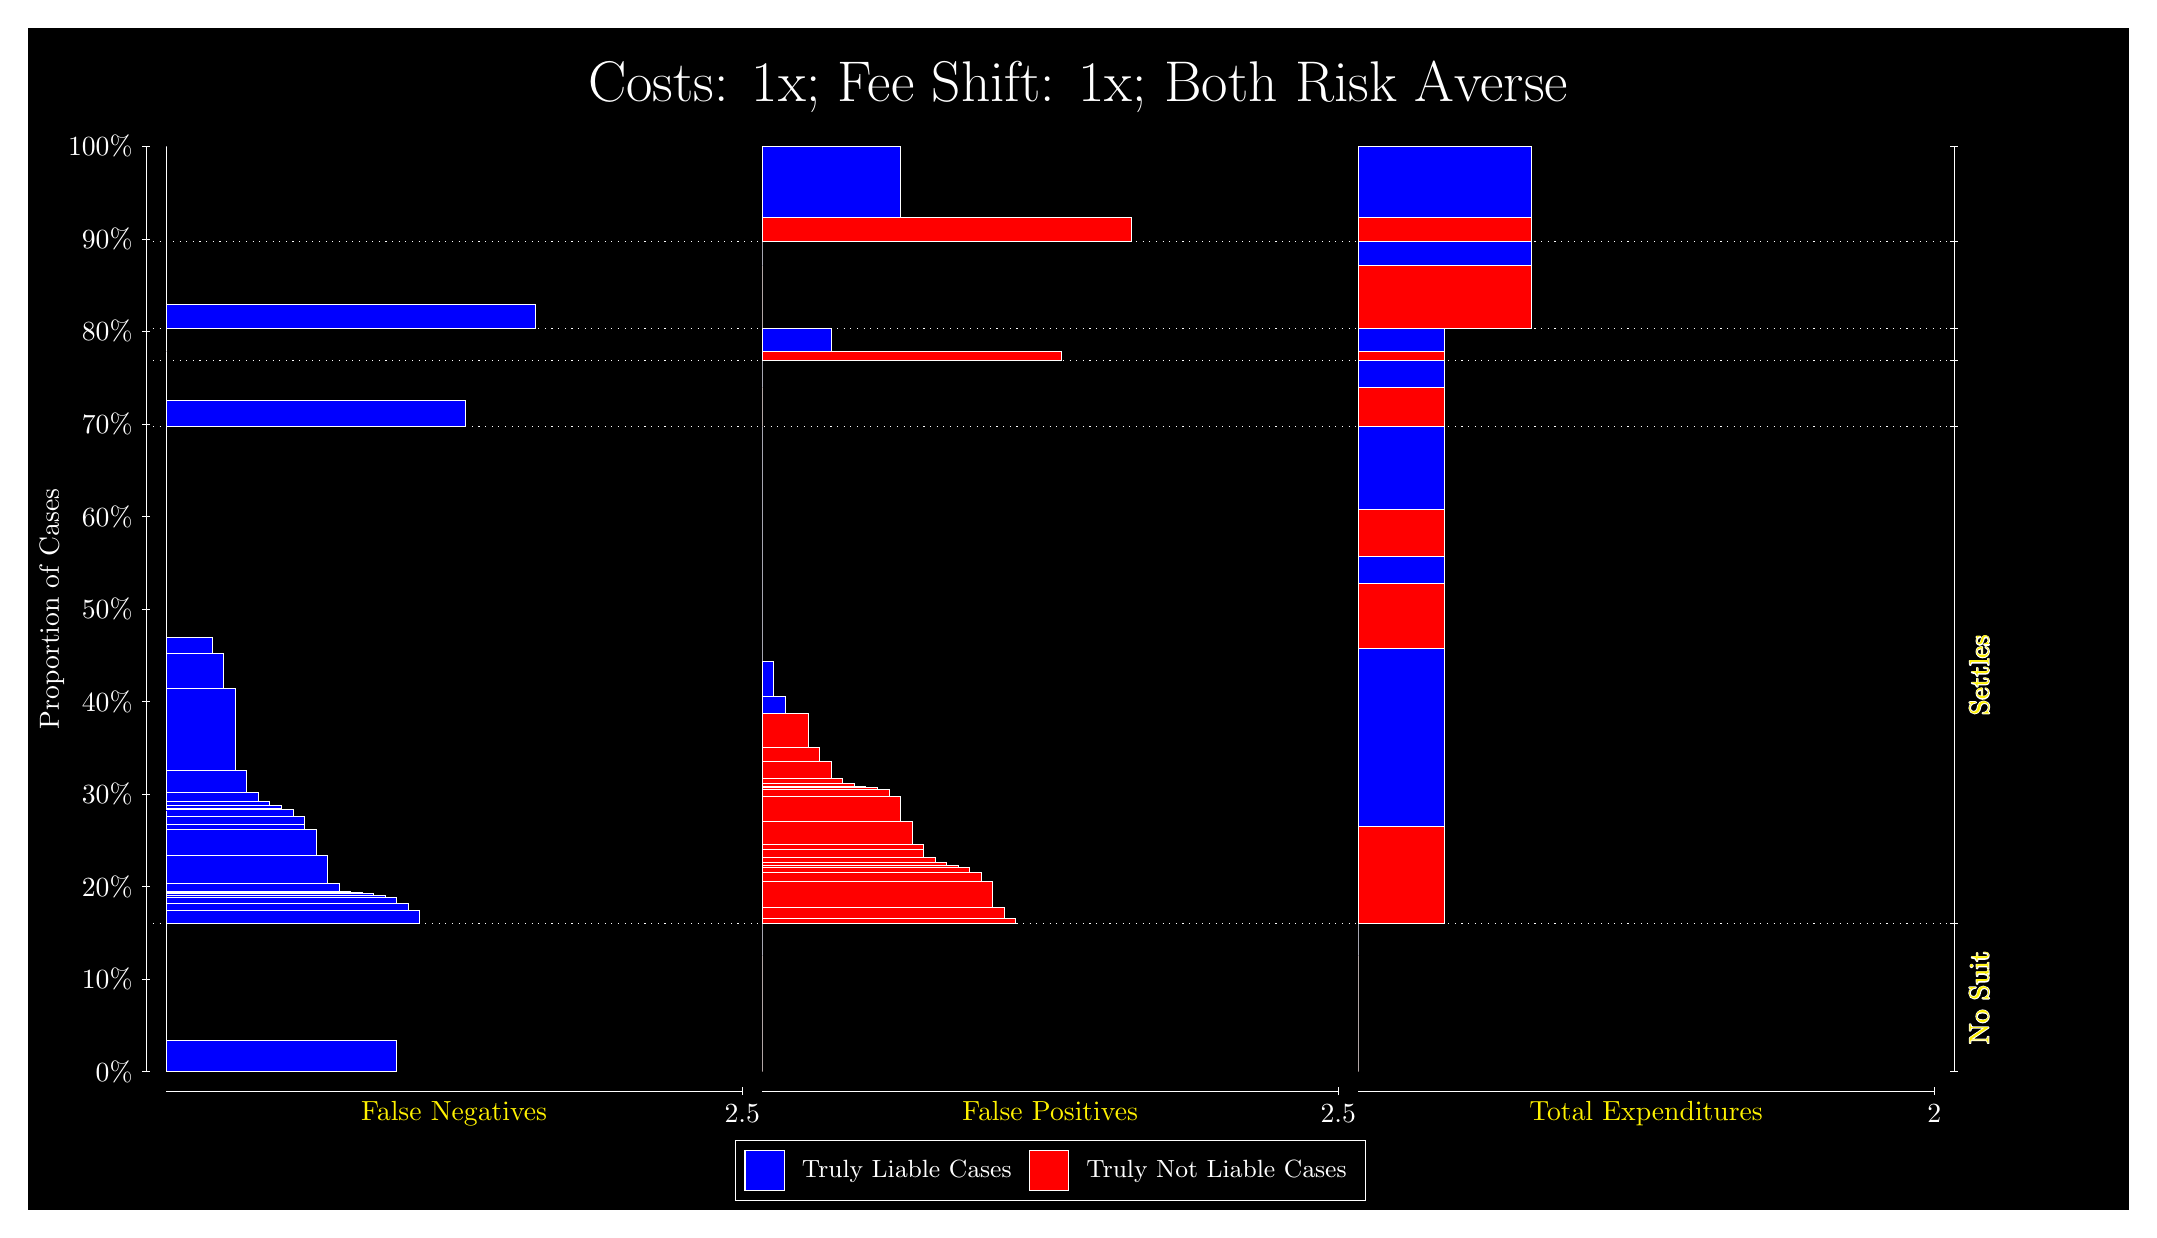
\begin{tikzpicture}
\draw[fill=black] (0,0) rectangle (26.667,15);
\draw[text=white] (0,13.5) rectangle (26.667,15) node[midway] {\huge Costs: 1x; Fee Shift: 1x; Both Risk Averse};
\draw[white, very thin] (1.5,1.75) -- (1.5,13.5);
\node[rotate=90, text=white, anchor=center] at (0.3, 7.625) {Proportion of Cases};
\draw[white, very thin] (1.45,1.75) -- (1.55,1.75);
\node[text=white, anchor=east] at (1.45, 1.75) {0\%};
\draw[white, very thin] (1.45,2.925) -- (1.55,2.925);
\node[text=white, anchor=east] at (1.45, 2.925) {10\%};
\draw[white, very thin] (1.45,4.1) -- (1.55,4.1);
\node[text=white, anchor=east] at (1.45, 4.1) {20\%};
\draw[white, very thin] (1.45,5.275) -- (1.55,5.275);
\node[text=white, anchor=east] at (1.45, 5.275) {30\%};
\draw[white, very thin] (1.45,6.45) -- (1.55,6.45);
\node[text=white, anchor=east] at (1.45, 6.45) {40\%};
\draw[white, very thin] (1.45,7.625) -- (1.55,7.625);
\node[text=white, anchor=east] at (1.45, 7.625) {50\%};
\draw[white, very thin] (1.45,8.8) -- (1.55,8.8);
\node[text=white, anchor=east] at (1.45, 8.8) {60\%};
\draw[white, very thin] (1.45,9.975) -- (1.55,9.975);
\node[text=white, anchor=east] at (1.45, 9.975) {70\%};
\draw[white, very thin] (1.45,11.15) -- (1.55,11.15);
\node[text=white, anchor=east] at (1.45, 11.15) {80\%};
\draw[white, very thin] (1.45,12.325) -- (1.55,12.325);
\node[text=white, anchor=east] at (1.45, 12.325) {90\%};
\draw[white, very thin] (1.45,13.5) -- (1.55,13.5);
\node[text=white, anchor=east] at (1.45, 13.5) {100\%};

\draw[white, very thin] (24.457,1.75) -- (24.457,13.5);
\draw[white, very thin] (24.407,1.75) -- (24.507,1.75);
\node[anchor=west] at (24.407, 1.75) {};
\draw[white, very thin] (24.407,3.629) -- (24.507,3.629);
\node[anchor=west] at (24.407, 3.629) {};
\draw[white, very thin] (24.407,9.9414) -- (24.507,9.9414);
\node[anchor=west] at (24.407, 9.9414) {};
\draw[white, very thin] (24.407,10.777) -- (24.507,10.777);
\node[anchor=west] at (24.407, 10.777) {};
\draw[white, very thin] (24.407,11.187) -- (24.507,11.187);
\node[anchor=west] at (24.407, 11.187) {};
\draw[white, very thin] (24.407,12.29) -- (24.507,12.29);
\node[anchor=west] at (24.407, 12.29) {};
\draw[white, very thin] (24.407,13.5) -- (24.507,13.5);
\node[anchor=west] at (24.407, 13.5) {};

\draw[white, very thin, fill=blue] (1.75,1.75) rectangle (4.6775,2.1529);
\draw[white, very thin, fill=red] (1.75,2.1529) rectangle (1.75,3.629);
\draw[white, very thin, fill=blue] (1.75,3.629) rectangle (4.9703,3.8034);
\draw[white, very thin, fill=blue] (1.75,3.8034) rectangle (4.8239,3.8819);
\draw[white, very thin, fill=blue] (1.75,3.8819) rectangle (4.6775,3.9606);
\draw[white, very thin, fill=blue] (1.75,3.9606) rectangle (4.5312,3.988);
\draw[white, very thin, fill=blue] (1.75,3.988) rectangle (4.3848,4.0111);
\draw[white, very thin, fill=blue] (1.75,4.0111) rectangle (4.2384,4.0261);
\draw[white, very thin, fill=blue] (1.75,4.0261) rectangle (4.092,4.0295);
\draw[white, very thin, fill=blue] (1.75,4.0295) rectangle (4.092,4.042);
\draw[white, very thin, fill=blue] (1.75,4.042) rectangle (3.9457,4.1415);
\draw[white, very thin, fill=blue] (1.75,4.1415) rectangle (3.7993,4.4957);
\draw[white, very thin, fill=blue] (1.75,4.4957) rectangle (3.6529,4.8222);
\draw[white, very thin, fill=blue] (1.75,4.8222) rectangle (3.5065,4.895);
\draw[white, very thin, fill=blue] (1.75,4.895) rectangle (3.5065,4.9967);
\draw[white, very thin, fill=blue] (1.75,4.9967) rectangle (3.3602,5.076);
\draw[white, very thin, fill=blue] (1.75,5.076) rectangle (3.3602,5.0768);
\draw[white, very thin, fill=blue] (1.75,5.0768) rectangle (3.2138,5.09);
\draw[white, very thin, fill=blue] (1.75,5.09) rectangle (3.2138,5.1271);
\draw[white, very thin, fill=blue] (1.75,5.1271) rectangle (3.0674,5.1768);
\draw[white, very thin, fill=blue] (1.75,5.1768) rectangle (2.921,5.3026);
\draw[white, very thin, fill=blue] (1.75,5.3026) rectangle (2.7746,5.5813);
\draw[white, very thin, fill=blue] (1.75,5.5813) rectangle (2.6283,6.612);
\draw[white, very thin, fill=blue] (1.75,6.612) rectangle (2.4819,7.0607);
\draw[white, very thin, fill=blue] (1.75,7.0607) rectangle (2.3355,7.2703);
\draw[white, very thin, fill=red] (1.75,7.2703) rectangle (1.75,9.9414);
\draw[white, very thin, fill=blue] (1.75,9.9414) rectangle (5.5558,10.28);
\draw[white, very thin, fill=red] (1.75,10.28) rectangle (1.75,10.777);
\draw[white, very thin, fill=red] (1.75,10.777) rectangle (1.75,10.896);
\draw[white, very thin, fill=blue] (1.75,10.896) rectangle (1.75,11.187);
\draw[white, very thin, fill=blue] (1.75,11.187) rectangle (6.4341,11.492);
\draw[white, very thin, fill=red] (1.75,11.492) rectangle (1.75,12.29);
\draw[white, very thin, fill=red] (1.75,12.29) rectangle (1.75,12.605);
\draw[white, very thin, fill=blue] (1.75,12.605) rectangle (1.75,13.5);
\draw[white, very thin, fill=red] (9.3189,1.75) rectangle (9.3189,3.2261);
\draw[white, very thin, fill=blue] (9.3189,3.2261) rectangle (9.3189,3.629);
\draw[white, very thin, fill=red] (9.3189,3.629) rectangle (12.539,3.6991);
\draw[white, very thin, fill=red] (9.3189,3.6991) rectangle (12.393,3.8367);
\draw[white, very thin, fill=red] (9.3189,3.8367) rectangle (12.246,4.1722);
\draw[white, very thin, fill=red] (9.3189,4.1722) rectangle (12.1,4.2784);
\draw[white, very thin, fill=red] (9.3189,4.2784) rectangle (11.954,4.3379);
\draw[white, very thin, fill=red] (9.3189,4.3379) rectangle (11.807,4.3742);
\draw[white, very thin, fill=red] (9.3189,4.3742) rectangle (11.661,4.4015);
\draw[white, very thin, fill=red] (9.3189,4.4015) rectangle (11.661,4.411);
\draw[white, very thin, fill=red] (9.3189,4.411) rectangle (11.515,4.4117);
\draw[white, very thin, fill=red] (9.3189,4.4117) rectangle (11.515,4.4765);
\draw[white, very thin, fill=red] (9.3189,4.4765) rectangle (11.368,4.5663);
\draw[white, very thin, fill=red] (9.3189,4.5663) rectangle (11.368,4.6347);
\draw[white, very thin, fill=red] (9.3189,4.6347) rectangle (11.222,4.9318);
\draw[white, very thin, fill=red] (9.3189,4.9318) rectangle (11.075,5.2477);
\draw[white, very thin, fill=red] (9.3189,5.2477) rectangle (10.929,5.3373);
\draw[white, very thin, fill=red] (9.3189,5.3373) rectangle (10.783,5.354);
\draw[white, very thin, fill=red] (9.3189,5.354) rectangle (10.636,5.3621);
\draw[white, very thin, fill=red] (9.3189,5.3621) rectangle (10.636,5.3698);
\draw[white, very thin, fill=red] (9.3189,5.3698) rectangle (10.49,5.4141);
\draw[white, very thin, fill=red] (9.3189,5.4141) rectangle (10.344,5.4796);
\draw[white, very thin, fill=red] (9.3189,5.4796) rectangle (10.197,5.6906);
\draw[white, very thin, fill=red] (9.3189,5.6906) rectangle (10.051,5.874);
\draw[white, very thin, fill=red] (9.3189,5.874) rectangle (9.9044,6.3001);
\draw[white, very thin, fill=blue] (9.3189,6.3001) rectangle (9.6116,6.5097);
\draw[white, very thin, fill=blue] (9.3189,6.5097) rectangle (9.4652,6.9585);
\draw[white, very thin, fill=blue] (9.3189,6.9585) rectangle (9.3189,9.9414);
\draw[white, very thin, fill=red] (9.3189,9.9414) rectangle (9.3189,10.439);
\draw[white, very thin, fill=blue] (9.3189,10.439) rectangle (9.3189,10.777);
\draw[white, very thin, fill=red] (9.3189,10.777) rectangle (13.125,10.896);
\draw[white, very thin, fill=blue] (9.3189,10.896) rectangle (10.197,11.187);
\draw[white, very thin, fill=red] (9.3189,11.187) rectangle (9.3189,11.984);
\draw[white, very thin, fill=blue] (9.3189,11.984) rectangle (9.3189,12.29);
\draw[white, very thin, fill=red] (9.3189,12.29) rectangle (14.003,12.605);
\draw[white, very thin, fill=blue] (9.3189,12.605) rectangle (11.075,13.5);
\draw[white, very thin, fill=red] (16.888,1.75) rectangle (16.888,3.2261);
\draw[white, very thin, fill=blue] (16.888,3.2261) rectangle (16.888,3.629);
\draw[white, very thin, fill=red] (16.888,3.629) rectangle (17.986,4.8697);
\draw[white, very thin, fill=blue] (16.888,4.8697) rectangle (17.986,7.1202);
\draw[white, very thin, fill=red] (16.888,7.1202) rectangle (17.986,7.9488);
\draw[white, very thin, fill=blue] (16.888,7.9488) rectangle (17.986,8.2884);
\draw[white, very thin, fill=red] (16.888,8.2884) rectangle (17.986,8.8902);
\draw[white, very thin, fill=blue] (16.888,8.8902) rectangle (17.986,9.9414);
\draw[white, very thin, fill=red] (16.888,9.9414) rectangle (17.986,10.439);
\draw[white, very thin, fill=blue] (16.888,10.439) rectangle (17.986,10.777);
\draw[white, very thin, fill=red] (16.888,10.777) rectangle (17.986,10.896);
\draw[white, very thin, fill=blue] (16.888,10.896) rectangle (17.986,11.187);
\draw[white, very thin, fill=red] (16.888,11.187) rectangle (19.083,11.984);
\draw[white, very thin, fill=blue] (16.888,11.984) rectangle (19.083,12.29);
\draw[white, very thin, fill=red] (16.888,12.29) rectangle (19.083,12.605);
\draw[white, very thin, fill=blue] (16.888,12.605) rectangle (19.083,13.5);
\draw[white, dotted] (1.5,3.629) -- (24.457,3.629);
\draw[white, dotted] (1.5,9.9414) -- (24.457,9.9414);
\draw[white, dotted] (1.5,10.777) -- (24.457,10.777);
\draw[white, dotted] (1.5,11.187) -- (24.457,11.187);
\draw[white, dotted] (1.5,12.29) -- (24.457,12.29);
\draw[white, very thin] (1.75,1.5) -- (9.0689,1.5);
\node[text=yellow, anchor=north] at (5.4094, 1.5) {False Negatives};
\draw[white, very thin] (9.0689,1.45) -- (9.0689,1.55);
\node[text=white, anchor=north] at (9.0689, 1.45) {2.5};

\draw[white, very thin] (9.3189,1.5) -- (16.638,1.5);
\node[text=yellow, anchor=north] at (12.978, 1.5) {False Positives};
\draw[white, very thin] (16.638,1.45) -- (16.638,1.55);
\node[text=white, anchor=north] at (16.638, 1.45) {2.5};

\draw[white, very thin] (16.888,1.5) -- (24.207,1.5);
\node[text=yellow, anchor=north] at (20.547, 1.5) {Total Expenditures};
\draw[white, very thin] (24.207,1.45) -- (24.207,1.55);
\node[text=white, anchor=north] at (24.207, 1.45) {2};

\node[text=yellow, centered, rotate=90] at (24.777, 2.6895) {\contour{white}{No Suit}};
\node[text=yellow, centered, rotate=90] at (24.777, 6.7852) {\contour{white}{Settles}};





\draw (12.978300999999998,1.5) node[draw=none] (baseCoordinate) {};
\begin{scope}[align=center]
        \matrix[scale=0.5, draw=white, below=0.5cm of baseCoordinate, nodes={draw}, column sep=0.1cm]{
            \node[rectangle, draw, minimum width=0.5cm, minimum height=0.5cm, fill=blue] {}; &
            \node[draw=none, font=\small, text=white] (B) {Truly Liable Cases}; &
            \node[rectangle, draw, minimum width=0.5cm, minimum height=0.5cm, fill=red] {}; &
            \node[draw=none, font=\small, text=white] (B) {Truly Not Liable Cases}; \\
            };
\end{scope}

\end{tikzpicture}
\end{document}